% Latex template
\documentclass[
	10pt, % Default font size, values between 10pt-12pt are allowed
	%letterpaper, % Uncomment for US letter paper size
	spanish, % Uncomment for Spanish
]{fphw}

% Template-specific packages
\usepackage[utf8]{inputenc} % Required for inputting international characters
\usepackage[T1]{fontenc} % Output font encoding for international characters
\usepackage{mathpazo} % Use the Palatino font
\usepackage{graphicx} % Required for including images
\usepackage{booktabs} % Required for better horizontal rules in tables

\usepackage{listings} % Required for insertion of code

\usepackage{enumerate} % To modify the enumerate environment
\usepackage{listings}

% titles 

\title{Práctica 1: Modulacións dixitais}

\author{Miguel Blanco Godón}

\date{26 de marzo do 2021}

\institute{Universidade da Coruña \\ Facultade de Informática} 

\class{Software de comunicacións (Enxeñaría de computadores)}

\professor{Óscar Fresnedo Arias} 

% actual document

\begin{document}

\maketitle 

\section*{Introdución}
O obxectivo desta práctica é a avaliación das modulacións do estándar IEEE 802.11n cando son transmitidas por canles AWGN. O método de avaliación será a simulación do sistema en Matlab.
Concretamente, as modulacións avaliadas son 2-PSK, 4-PSK, 16-QAM, 64-QAM.
\section*{Arquitectura do sistema}
O sistema está composto por tres partes, un modulador dixital, unha canle AWGN e un demodulador dixital. Un sistema de comunicación está formado por, como mínimo, un emisor, unha canle de comunicación en un receptor. O modulador forma parte do emisor, a canle AWGN é o medio para a comunicación e o demodulador forma parte do receptor.
\subsection*{Modulador dixital}
É a primeira parte do sistema, a cal que encarga de convirtir o fluxo de bits un conxunto de símbolos dependentes da modulación. Para iso basámonos na representación discreta equivalente, a través dun método denominado \textit{representación vectorial de sinais}. Este método, que forma parte do análise espacial de sinais, foi desenvolvido primeiramente por V.A.Kotel'nikov en 1947. A idea consiste en representar cada elemento dun conxunto de sinais transmitidas mediante un vector N-dimensional, sendo N o número de funcións básicas ortonormais necesarias para unha representación xeométrica única dos sinais transmitidos.
Un parámetro importante na modulación, aparte do tipo, é o número de niveis. O número de niveis dunha modulación dánolo o valor de M, o número de sinais necesarias, e implica que cada símbolo conterá  a información de $log_2{M}$ bits.
As bases a usar dependen de cada modulación:
\begin{itemize}
\item \textbf{Phase Shift Keying (PSK)}: modifica a fase nunha portadora de frecuencia constante.
\item \textbf{Quadrature Amplitude Modulation (QAM)}: modifica a fase e a amplitude da sinal portadora. 
\end{itemize}
\subsection*{Canle AWGN}
En comunicacións, unha canle é un medio de transmisión a través dos cales viaxa a información. Neste caso, o estándar utilizado é un estándar de comunicación inalámbrico, polo que o medio de transmisión é o aire. Nesta práctica simúlase un canle AWGN (Additive White Gaussian Noise) debido a que é un tipo de canle que se asemella a moitos fenómenos de interferencia na vida real, como pode ser o ruído térmico. A canle modélase como: $\vec{r} = \vec{s} + \vec{n}$, onde o sinal recibido é igual ao sinal emitido máis a interferencia da canle.
\subsection*{Demodulador}
O demodulador forma parte do receptor, e o seu traballo é recuperar o fluxo de bits transmitido a partir da información que porta a portadora. 
Para isto o demodulador debe estimar cal é o símbolo transmitido, e despois convertir os símbolos a bits. Para que o demodulador funcione, debe ser compatible co modulador. 
\section*{Implementación en Matlab a través do modelo discreto equivalente}
Para a implementación separo código en sete módulos. Ilústrase o funcionamento a partir dun caso de proba de 12 bits:
\begin{itemize}
\item \textbf{modulate.m}: implementa o modulador. En función dos parámetros de entrada, establece a dimensión das bases da modulación e modula o fluxo de bits a partir dun vector de símbolos adecuado a cada modulación. 
\begin{lstlisting}[language=matlab]
% modulation type checking and modulation computation
if (strcmp(modulation_type, "PAM"))
	modulation = pam(modulation_levels, ordering);
	dimension = 1;
	complex = false;
elseif (strcmp(modulation_type, "PSK"))
	modulation = psk(modulation_levels, ordering);
	dimension = 2;
	complex = true;
elseif (strcmp(modulation_type, "QAM"))
	modulation = qam(modulation_levels, ordering);
	dimension = 2;
	complex = true;
else
	error('Unsupported modulation type. Supported modulations: PAM, PSK, QAM');
end
% reshaping matrix so that it fits the number of bits/symbol
input_matrix = reshape(input_bitstream, log2(modulation_levels), []);
% modulation_computation
modulated_stream = modulation(bi2de(input_matrix', 'left-msb')+1);
\end{lstlisting}
Como se pode observar no código, ao primeiro obtense o vector de símbolos para a modulación. Despois, reorganízase o vector como unha matriz de dúas dimensións, de tal xeito que en cada columna quede o equivalente a un símbolo, e por último, indexamos o vector de símbolos da modulación a partir dos da matriz;que pasa a ser outro vector debido a que se fai unha conversión por columnas a decimal, o que nos dá a posición (comezando a contar dende 0) do símbolo no vector de símbolos da modulación. Súmaselle 1 xa que Matlab indexa dende 1 ata N. Así obtense o vector de símbolos modulados. Todo este proceso pódese facer chamando á función do módulo \textit{modulate}:
\begin{lstlisting}[language=matlab]
bits = randn(1,12)>0.5

bits =

  1x12 logical array

   0   0   0   0   1   0   0   1   0   0   1   1

modulate(bits, uint8(4), "PAM", 'bin')

ans =

    -3    -3     1    -1    -3     3
\end{lstlisting}
\item \textbf{awgn.m}: neste módulo emúlase a canle AWGN en base a dous parámetros, a dimensión da modulación (se 1, só ruido real, se 2, real e complexo). Como a canle é de ruido aditivo, pódese calcular simplemente mediante a adición de vectores. O ruido créase en relación a un parámetro de simulación, $N_0$, e segue unha distribución gaussiana de $\mu = 0$ e $\sigma = \frac{N_0}{2}$.
O parámetro $N_0$ calcúlase neste módulo a partires do valor de $\frac{E_b}{N_0}$.
\begin{lstlisting}[language=matlab]
% compute symbol energy
symbol_energy = mean(abs(modulated_stream).^2);
% compute bit energy
bit_energy = symbol_energy / double(bits_per_symbol);
% compute N0
N0 = bit_energy / (10^(dbEbN0/10));
if (dimension == 1)
	% creates gaussian noise with mean 0 and tipic deviation N0/2
	noise = sqrt(N0/2) * randn(size(modulated_stream));
	% adds noise to the modulated stream
	noisy_modulated_stream = modulated_stream + noise;
elseif ((dimension == 2) & complex)
	% creates gaussian noise with mean 0 and tipic deviation N0/2
	real_noise = sqrt(N0/2) * randn(size(modulated_stream));
	imag_noise = sqrt(N0/2) * randn(size(modulated_stream))*1j;
	noisy_modulated_stream = modulated_stream + real_noise + imag_noise;
end
\end{lstlisting}
Aquí vese cun exemplo a partir do vector de símbolos modulados anterior:
\begin{lstlisting}[language=matlab]
m =

    -3    -3     1    -1    -3     3

[recv, e_bit, e_simbolo, n0] = awgn(m, uint8(log2(4)), uint8(1), false, 5)

recv =

   -4.9284   -2.2008    1.8532   -1.6854   -2.9138    1.3956


e_bit =

    3.1667


e_simbolo =

    6.3333


n0 =

    1.0014
\end{lstlisting}
\item \textbf{demodulate.m}: o demodulador realiza exactamente a operación inversa ao modulador, partindo dende o mesmo vector de símbolos da modulación.
\begin{lstlisting}[language=matlab]
% modulation type checking and modulation computation
if (strcmp(modulation_type, "PAM"))
	modulation = pam(modulation_levels, ordering);
elseif (strcmp(modulation_type, "PSK"))
	modulation = psk(modulation_levels, ordering);
elseif (strcmp(modulation_type, "QAM"))
	modulation = qam(modulation_levels, ordering);
else
	error('Unsupported modulation type. Supported modulations: PAM, PSK, QAM');
end
% vector replication to parallel contrast of input stream
input_matrix = repmat(modulated_stream, length(modulation), 1);
% correlate modulated input with modulation
input_matrix = input_matrix - modulation.';
% get the position to which symbol demodulates
[~, pos] = min(abs(input_matrix));
% returning bitstream
demodulated_stream = logical(reshape(de2bi(pos-1, 'left-msb')', 1, []));
\end{lstlisting}
Do mesmo xeito ca no modulador, obtense o vector de símbolos da modulación. Replícanse as filas do vector de símbolos para poder calcular a distancia euclídea a todos os símbolos cunha soa instrución. Despois extráese a posición do símbolo na constelación a través do mínimo, que Matlab faino por columnas, e por último simplemente se desfai a tradución, pasando a binario as posicións correspondentes. Pódese observar o seguinte exemplo:
\begin{lstlisting}[language=matlab]
demodulate(recv, uint8(4), "PAM", 'bin')

ans =

  1x12 logical array

   0   0   0   0   1   0   0   1   0   0   1   0
\end{lstlisting}
Onde se pode observar que houbo un erro da demodulación.
\item \textbf{transmit.m}: é unha abstracción do sistema, que xa fai todo o proceso de modulación, transmisión pola canle e demodulación.
\item \textbf{pam.m}: devolve un vector cos símbolos da modulación M-PAM. Concretamente, calcula os vectores a partires da expresión $s_i = 2k + 1 - M \quad \forall k = 0, ..., M-1$.
\item \textbf{psk.m}: devolve un vector cos símbolos da modulación M-PSK. Concretamente, calcula os vectores a partires da expresión $s_i = \sqrt{\frac{1}{2}} cos(\theta_k) + \sqrt{\frac{1}{2}} sen(\theta_k)j \quad \forall k = 0,...,M-1$ onde $\theta_k = \frac{2\pi k}{M}$.
\item \textbf{qam.m}: devolve un vector cos símbolos da modulación M-QAM. Bótase man da función \textit{qammod} do \textit{Communications toolbox} de Matlab. 
\end{itemize}
Isto todo xúntase no script \textit{p1.m} no cal se executan as transmisións e xéranse as figuras. Para o cómputo das BER empíricas, simplemente se dividen o número de erros de cadra transmisión entre o número de bits transmitidos. Para o cómputo das BER teóricas, por outra banda, realízase por medio de substitucións nas fórmulas teóricas dos datos concretos para cada transmisión.
\section*{Resultados}
O script xera 9 gráficas. As primeiras 5 figuras amosan as BER empíricas e teóricas das modulacións 4-PAM, BPSK, QPSK, 16-QAM, 64-QAM. Nas 4 restantes temos:
\begin{itemize}
\item \textbf{Figura 6}: BER para BPSK, QPSK, 16-QAM, 64-QAM utilizando todas Gray Mapping.
\begin{figure}[htb]
\centering 
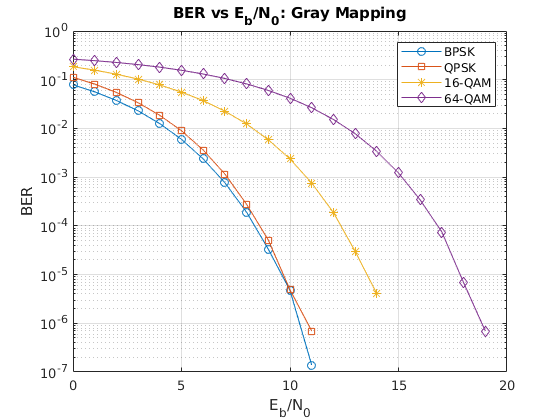
\includegraphics{figura6.png}
\caption{Figura 6}
\end{figure}
\item \textbf{Figura 7}: BER para BPSK natural, QPSK con e sen Gray Mapping e a BER teórica de QPSK.
\begin{figure}[htb]
\centering 
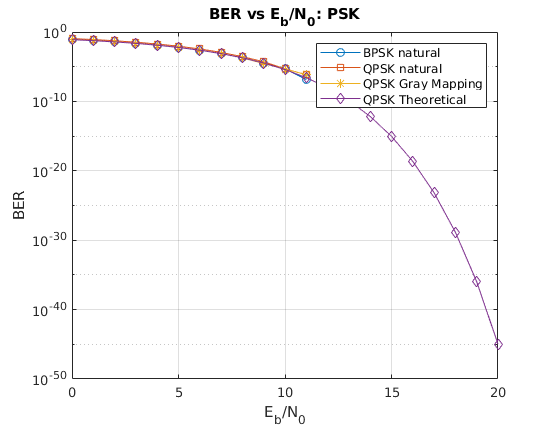
\includegraphics{figura7.png}
\caption{Figura 6}
\end{figure}
\item \textbf{Figura 8}: BER para 16-QAM con e sen Gray Mapping e a súa correspondente BER teórica.
\begin{figure}[htb]
\centering 
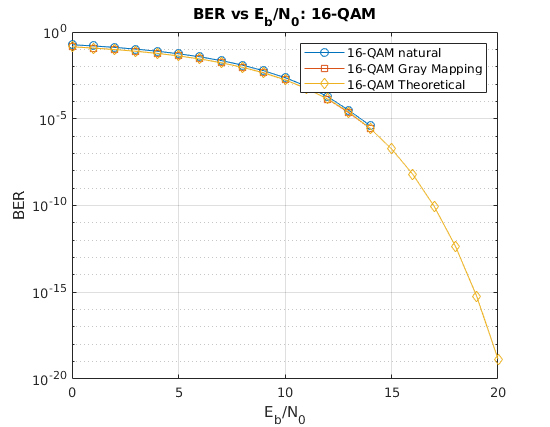
\includegraphics{figura8.png}
\caption{Figura 6}
\end{figure}
\item \textbf{Figura 9}: BER para 64-QAM con e sen Gray Mapping e a súa BER teórica.
\begin{figure}[htb]
\centering 
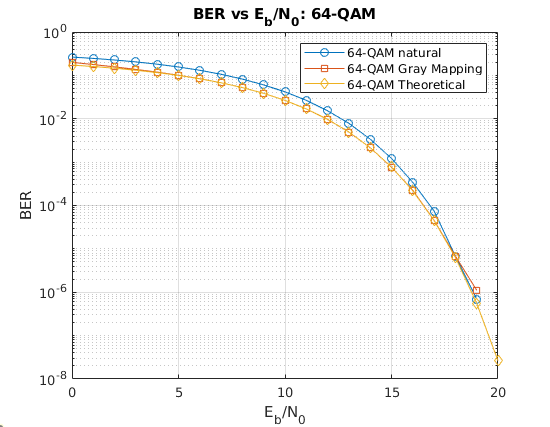
\includegraphics{figura9.png}
\caption{Figura 6}
\end{figure}
\end{itemize}
De entre todas as figuras podemos salientar dúas cousas: primeiro, que cantos menos niveis teña unha modulación, menor a súa probabilidade de erro de símbolo e, por tanto, mellor rendemento; e segundo, que ao utilizar Gray Mapping para minimizar o erro de bit (malia non modificar o erro de símbolo) obtemos o mellor rendemento posíbel, xa que coincide coa probabilidade de erro teórica. Outro aspecto interesante é o relacionado co parámetro de simulación $E_b/N_0$. Este parámetro é unha medida normalizada da «relación sinal ruido» da canle, polo cal canto maior sexa a «cantidade de sinal» respecto á «cantidade de ruido», menos relevante será a interferencia da canle AWGN nos símbolos transmitidos, derivando en unha menor tasa de fallo. En síntese, o valor de $E_b/N_0$ é inversamente proporcional á tasa de erro.
Os valores concretos de BER vense completamente ao executar o script, debido a que se pode ampliar.
Tamen podemos caer na tentación de pensar que PSK é o mellor esquema de modulación, debido a que ten a menor tasa de erros, pero isto só se cumpre se temos poucos niveis da modulación, como se pode observar nas «Figure 5» e «Figure 6».
\begin{figure}[htb]
\centering
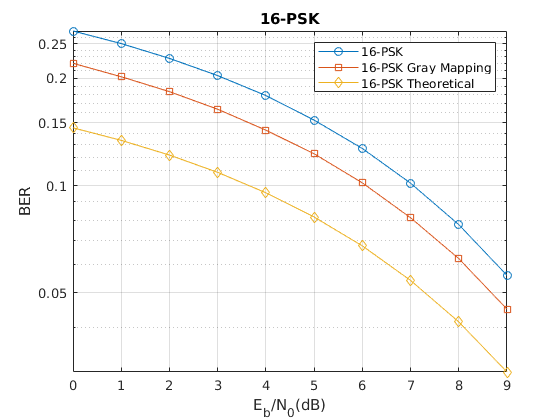
\includegraphics{16_psk.png}
\caption{Valores de BER para 16-PSK con e sen Gray Mapping}
\end{figure}
Este aumento tan drástico das tasas de erro en PSK débese á forma da constelación, pois aumentar o número de niveis, implica aumentar o número de símbolos veciños no mesmo espazo, polo cal dá maior tasa de erro, como se pode observar na imaxe das constelacións.
\begin{figure}[htb]
\centering
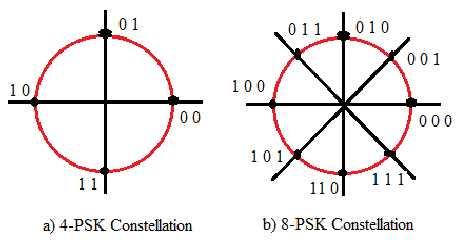
\includegraphics{4_8_psk_const.png}
\caption{Constelación de QPSK e 8-PSK. Pódese ver como ao aumentar M aumenta o número de símbolos sobre a circunferencia, pero non aumenta o tamaño da mesma, provocando que diminúa a separación e as colas de probabilidade de superpoñan máis.}
\end{figure}
\begin{figure}[htb]
\centering
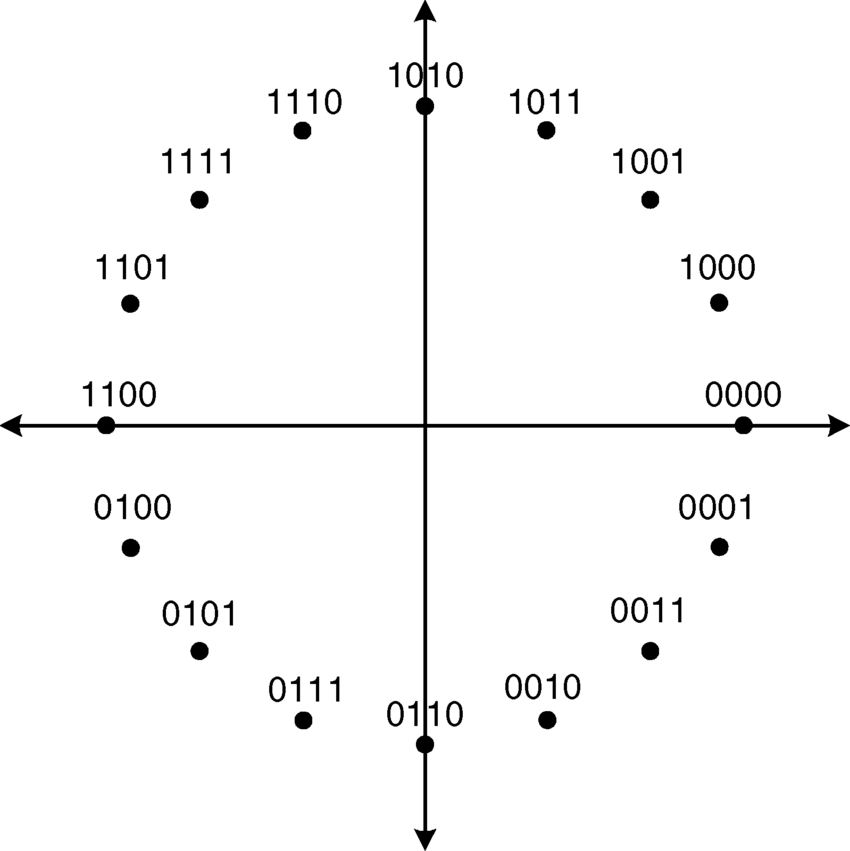
\includegraphics[scale=0.5]{psk_16_const.png}
\caption{Constelación da modulación 16-PSK}
\end{figure}
\section*{Conclusión}
Ante a vista dos resultados anteriores, vemos que o mellor esquema de modulación é PSK, sempre que traballemos con valores baixos de M. Pero podemos comprender o uso dos dous tipos de modulación tendo en conta que IEEE 802.11n é un estándar de comunicación inalámbrico. Hoxe en día, a maior parte dos usuarios conéctanse a redes inalámbricas dende dispositivos pequenos e portables, onde hai múltiples dispositivos de distintos propósitos emitindo ondas de radio, xa sexa para comunicarse ou como residuo. O método da modulación soluciona inconvenientes particularmente importantes neste medio, como o tema do tamaño dos dispositivos necesarios, pois a lonxitude de onda é inversamente proporcional á frecuencia ($\lambda = \frac{c}{f}$), o que permite dispoñer de antenas moi pequenas, que poden ser inseridas dentro de equipos informáticos compactos.\newline Ademais, cando medimos a calidade dunha comunicación, podemos medir dous parámetros:
\begin{itemize}
\item \textbf{Velocidadade da comunicación}: supoñendo un período de símbolo igual, a máis niveis de modulación, enviamos máis información na mesma unidade de tempo.
\item \textbf{Tasa de fallos}: en entornos de moito ruido, debemos usar modulacións que nos permitan obter baixas tasa de erros para valores baixos de $E_b/N_0$.
\end{itemize}
Tendo en conta iso, podemos ver que as modulacións BPSK e QPSK son moi boas para entornos con moita interferencia, porque son as que conseguen a menor tasa de fallos, sobre todo aplicando Gray Mapping, pero en entornos onde a interferencia sexa baixa podemos aumentar a velocidade da comunicación utilizando esquemas de modulación que nos permitan enviar moitos bits por símbolo con pouca tasa de erros, onde son particularmente boas as modulacións QAM. 
\end{document}
